
\section{Introducción}
El diseño, desarrollo, fabricación, armado, simulación y lanzamiento de cohetes, no es una tarea
sencilla ni es repetida en intervalos de cortos de tiempo, al contrario, suelen llevar décadas y una
fuerte inversión para que sean posibles estos logros. Cuando se completa el desarrollo de estos vehiculos son lanzados y generalmente una vez completada la misión pasan a ser parte de la basura espacial o reeingresan a la atmosfera terrestre sin posibilidad de reutilización. En los últimos años se ha buscado subsanar el costo incurrido por la incapacidad de volver a reutlizar el vehículo. Es allí donde nace el interés del desarrollo de vehículos reutilizables. Lo beneficios de un vehíclo reutilizable

\begin{itemize}
    \item El vehículo se puede reutilizar con mínimas intervenciones, minimizando el tiempo entre misiones
    \item Reducción de costos: Los cohetes reutilizables permiten que se utilicen los mismos vehículos para múltiples misiones, lo que reduce significativamente los costos de producción y operación.
    \item Mayor confiabilidad: Los cohetes reutilizables tienen un historial de éxito probado en múltiples misiones, lo que aumenta la confiabilidad y la seguridad en los lanzamientos.
    \item Flexibilidad: Los cohetes reutilizables son más flexibles y pueden ser utilizados para una variedad de misiones, lo que los hace más versátiles que los cohetes desechables.
    \item Reducción del impacto ambiental: La reutilización de cohetes reduce la cantidad de residuos y desechos generados por los lanzamientos.
    \item Innovación tecnológica: El desarrollo de cohetes reutilizables ha impulsado la innovación tecnológica en el campo de los cohetes y ha llevado a mejoras en la tecnología de propulsión y sistemas de recuperación.
\end{itemize}

\medskip

\medskip

El concepto de un vehículo VTVL es tan viejo como el primer alunizaje: despega verticalmente (como la mayoría de los cohetes
convencionales) y aterriza verticalmente con el objetivo de completar una misión. Esto supone una gran variante de ventajas, como ser una de
las más destacadas el reutilizamiento del vehículo, con todo lo que ello implica, logrando una
optimización de los costos, disminución de huella ecológica, y disminución del tiempo entre lanzamientos. Con solo agregar unos actuadores y el control correspondiente al vehículo se puede pasar de ser un cohete convencional a ser un VTVL y asi tener amplio dominio sobre donde aterrizará.

\medskip

\medskip

A baja escala, un vehículo que despega y aterriza por su cuenta tiene la capacidad de
superar cualquier obstáculo terrestre que se presente. Esto puede ser de gran utilidad en ambientes hostiles para el
ser humano, que esto se logre de manera rápida y efectiva podría ser la diferencia entre el
éxito o no de la misión.
Como ser el transporte de insumos médicos en tiempo real desde que un paciente lo requiere,
en zonas de acceso limitado.

\medskip

Una variante de estos vehículos se logra cuando se cierra el lazo de control obteniendosé un vehículo autónomo. La autonomía se refiere a la capacidad del vehículo para tomar decisiones y realizar tareas sin la necesidad de intervención humana durante la misión. La autonomía también incluye la capacidad del vehículo para realizar tareas adicionales, como la navegación y el mantenimiento de la trayectoria, la evitación de obstáculos y la toma de decisiones en tiempo real en función de los datos recopilados por los sensores del vehículo. En la última década hay un interés renovado en imágenes espaciales. Un vehículo VTVL, reutilizable autónomo, eléctrico podría adquirir imágenes para fines de sistemas de monitoreo y análisis geoespacial como hacen las empresas \textit{Ceres Imaging} y \textit{Martin UAV} con su vehículo V-BAT. Estas empresas dependen de vehículos autonomos no tripulados para obtener sus imágenes aéreas.

\medskip

%El vehículo una vez desarrollado y funcionando, puede servir de plataforma para diversos estudios de fenómenos de dinámica de fluidos, como ser, mediciones aerodinámicas, investigación del \textit{fuel sloshing} en vehículos con tanques esbeltos.

\medskip

Un vehículo de escala reducida provee la capacidad de testear sistemas de control. Si se pierde el vehículo ante una falla el costo total de perdidas seria mucho menor con respecto a un vehículo mas grande con sistemas caros y complejos. Al tener un sistema de control definido en términos de parámetros del vehículo, se podría escalar para luego ser probado en un vehículo mas grande. Siendo un sistema más chico y manipulable que el vehículo de escala grande se tornarían más fáciles las tareas de resolver los problemas de software y hardware de vuelo que surgieran durante las pruebas.

\medskip


Los sistemas de vehículos orbitales tienen sistemas complejos que deben ser testeados en una primera etapa mediante algún ensayo controlado. El vehículo que se desarrolla en el presente documento podría ser usado para tales fines como una plataforma para pruebas como ser el despliegue de una nariz o etapa, comprobación de sensores y actuadores a gran velocidad y con empuje variable.

\medskip

La tecnología VTVL permite a los cohetes de SpaceX aterrizar verticalmente después de su lanzamiento, en lugar de caer en el océano o en tierra y luego ser recuperados. La primera vez que SpaceX logró aterrizar con éxito un cohete Falcon 9 fue en diciembre de 2015, y desde entonces ha logrado muchos otros aterrizajes exitosos, tanto en plataformas en tierra como en barcos en el mar. El aterrizaje vertical de los cohetes de SpaceX es una hazaña técnica impresionante, ya que los cohetes deben desacelerar y estabilizarse en el aire antes de aterrizar de manera segura en una plataforma pequeña.


\begin{figure}[htb]
    \centering
    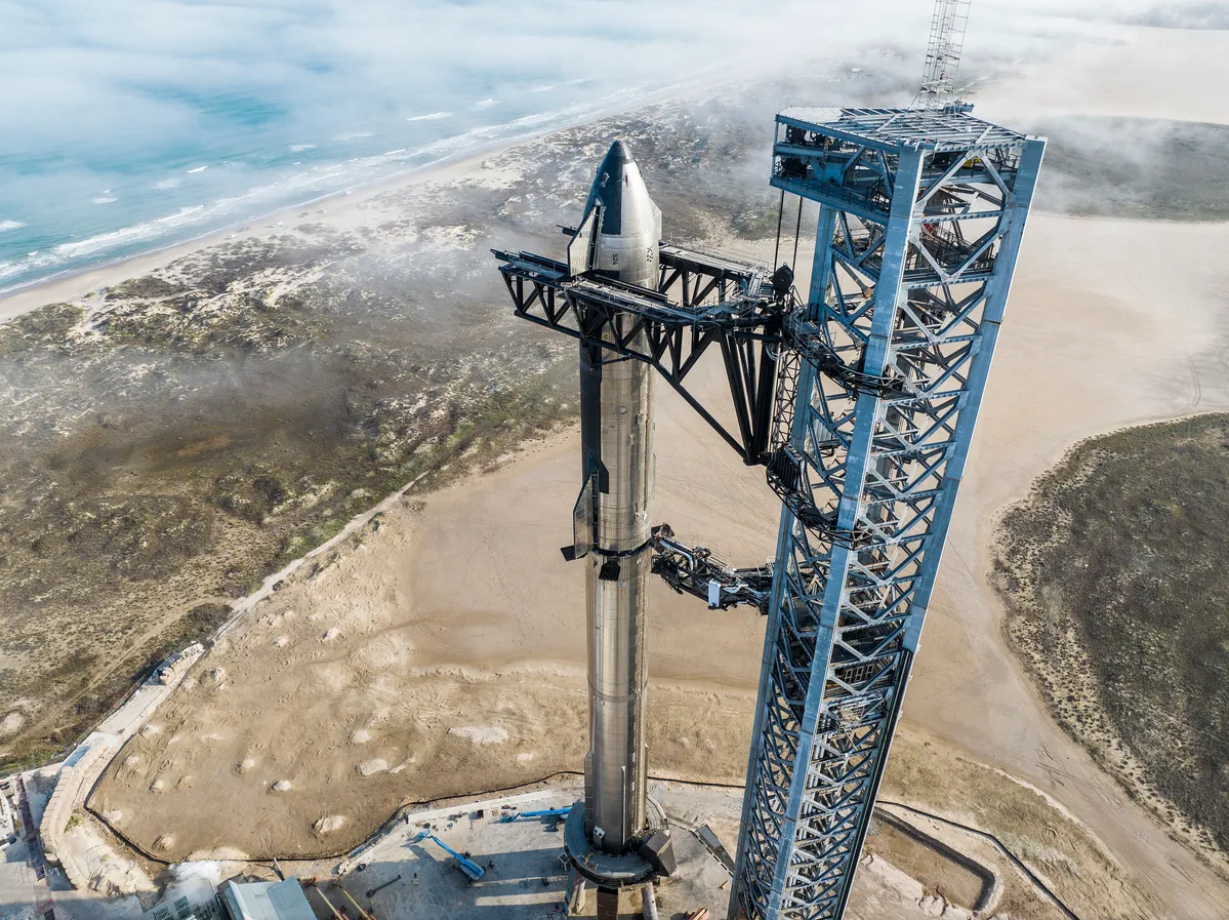
\includegraphics[width=0.8\linewidth]{fig/starhip2.png}
    \caption{Starship de SpaceX en rampa de lanzamiento.}
    \label{fig:starshipcool}
\end{figure}


Además de utilizar la tecnología VTVL en sus cohetes, SpaceX está trabajando en una nave espacial reutilizable llamada Starship, que utilizará esta tecnología para aterrizar en la Luna, Marte y otros destinos. La Starship también será capaz de realizar misiones terrestres y de corta duración, como vuelos turísticos suborbitales. La tecnología VTVL es una de las muchas innovaciones que SpaceX está utilizando para hacer que los viajes espaciales sean más asequibles y accesibles para más personas en el futuro.

\medskip

Otra organización que está apostando a la tecnología de lanzadores reutilizables es la ESA. Esta tiene un proyecto destinado a acelerar el desarrollo de tecnología de lanzadores reutilizables para las partes interesadas en el sector aeroespacial europeo. Se tiene pensado tener un lanzador reutilizable para 2030 llamado Ariane Next. Uno de los pasos a seguir antes de llegar a ese punto es el desarrollo del proyecto FROG. El proyecto FROG es un demostrador tecnológico para algoritmos de control y de métodos ágiles de proyectos \cite{rmili2019frog}.

\medskip

La ESA también ha estado trabajando en un proyecto llamado "Space Rider", que es una nave
espacial reutilizable que se lanzará al espacio en un cohete Vega-C. Una vez terminada la misión en órbita podrá volver a la tierra y aterrizar horizontalmente o verticalmente en modo VTVL. Space Rider se está diseñando como una
plataforma multipropósito para la realización de experimentos científicos y tecnológicos en órbita
terrestre baja LEO. Además, la ESA ha estado colaborando con empresas privadas europeas en el
desarrollo de cohetes reutilizables que utilizan este tipo de tecnologías. Como la empresa alemana Isar
Aerospace que está trabajando en el desarrollo de un cohete de lanzamiento de satélites reutilizable.

\begin{figure}[htb]
    \centering
    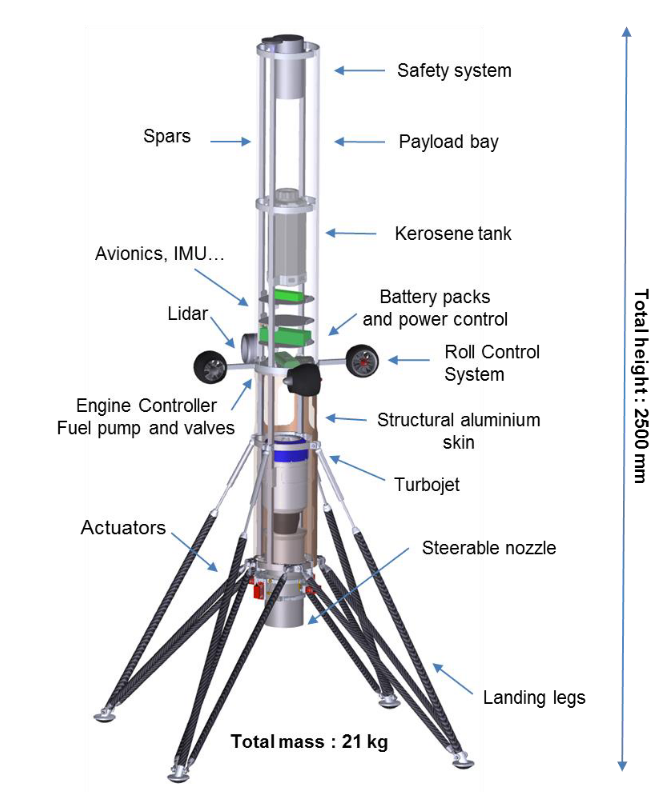
\includegraphics[width=0.8\linewidth]{fig/frogTArch.png}
    \caption{Arquitectura de FROG-T de la ESA \cite{rmili2019frog}.}
    \label{fig:frogtarch}
\end{figure}

\null\newpage
\clearpage

\section{Alcance de este proyecto}
Este documento propone el diseño, simulación, control y fabricación de un vehículo con capacidades VTVL, reutilizable, autonomo-- siendo un prototipo de baja escala. Este prototipo serviría como punta pie inicial para vehículos de escala mayor que puedan completar misiones espaciales. 

Se establecieron las siguientes etapas para el desarrollo del proyecto en el formulario de alta del proyecto 201--129 el 2 de mayo de 2020:
\begin{enumerate}
    \item Preparación inicial (3meses) [3]
    \begin{itemize}
        \item Teoría de sistema de control. Variables de estado.
        \item Proponer solución full state feedback con LQR + filtro Kalman.
        \item Práctica usando Simulink.
    \end{itemize}
    \item Diseño de sistema 3D (4 meses) [7]
    \begin{itemize}
        \item Selección del propulsor ducted fan.
        \item Diseño de estructura de cohete.
        \item Teoría de control automático.
        \item Diseño de control 3D.
    \end{itemize}
    \item Validación experimental del sistema de control (3 meses) [10]
    \begin{itemize}
        \item Seleccionar computadora de vuelo y componentes para el funcionamiento en la práctica.
        \item Manufactura de componentes del cohete.
        \item Puesta a prueba del sistema de control en cohete.
        \item Efectuar correcciones/ajustes al sistema de control.
    \end{itemize}
    \item Elaboración de informes
    \begin{itemize}
        \item Informe 1: Agosto 2020 -- Etapa 2.
        \item Informe 2: Diciembre 2020 -- Informe experimental.
        \item Informe 3: Enero 2021 -- Informe de diseño.
        \item Informe preliminar: Febrero 2021.
        \item Informe final: Marzo 2021 (considerando las correcciones previas realizadas por el tutor)
    \end{itemize}
\end{enumerate}

Basándose en los requisitos implícitos discutidos entre dos individuos con recursos limitados, se llevó a cabo un proyecto que desafió las convenciones establecidas en la industria. A diferencia de los proyectos realizados en entornos empresariales, que se basan en reglas establecidas y en la experiencia previa acumulada, este proyecto fue emprendido por personas sin experiencia en el control de un cohete VTVL y en su fabricación. Si bien al principio se establecieron ciertos requisitos para el proyecto, la falta de experiencia llevó a la imposibilidad de anticipar todos los desafíos que surgirían a lo largo del desarrollo del proyecto. Además, el equipo no estaba familiarizado con el ámbito del proyecto y por lo tanto se esperaban cambios significativos en el proceso de desarrollo.

La perseverancia y la determinación resultaron fundamentales para superar los constantes desafíos a lo largo del proyecto. La capacidad de adaptarse a los cambios fue fundamental para superar los obstáculos y alcanzar el éxito. La falta de experiencia técnica inicial parecía ser una barrera insuperable, pero el equipo demostró que el éxito puede ser alcanzado a través de la determinación y la perseverancia.

\subsection*{Requerimientos del proyecto}
Para poder llevar a cabo el proyecto del vehículo VTVL, reutilizable, autonomo a baja escala; fabricado por un equipo de dos personas con el presupuesto de un proyecto final de facultad se requiere lo siguiente:
\begin{itemize}
    \item Cumplir con el presupuesto establecido
    \item Que el tiempo de vuelo esté comprendido en un valor a 60 segundos
    \item Que soporte los aterrizajes necesarios para poder probar el sistema de control
    \item Capacidad de 1kg de payload
    \item Sistema de control que recupere de una perturbación delta-dirac de 15 grados de actitud en un eje a una altura de 1.5 metros durante funcionamiento
    \item Sistema de control completamente bajo el mando del equipo
    \item Capacidad de despegar y aterrizar en atmosfera terrestre
    \item Componentes utilizados en este proyecto sean disponibles comercialmente
\end{itemize}

Cabe destacar que antes del FROG, en la ESA se pasó por una etapa preliminar de desarrollo con un vehículo con prestaciones casi idénticas al vehículo que se va a detallar en este documento.



\section{Estudios}

\subsection{Agua como propelente}\label{ssec:propAgua}
El primer prototipo muy distante del diseño final perteneciente a este trabajo, consistía en un
recipiente a presión con agua, abulonado a un chasis, con un cardán y actuadores para poder redirigir el
empuje. 

\medskip

La figura~\ref{fig:bottlerocket} muestra los resultados de una simulación de un vehículo pequeño de aluminio con un recipiente a presión lleno en parte de agua y aire a 200 bar. La simulación considera masa variable y una transición isoentrópica del gas en el recipiente. En el mejor de los casos se llegaba a un tiempo de vuelo cercano a los 4 segundos, que no era adecuado para comprobar el sistema de control en nuestras condiciones. 

Para optimizar este problema se modificaba

\begin{itemize}
    \item Diámetro de la tobera -- más empuje vs. menos tiempo de vuelo controlado
    \item Volumen de agua -- más tiempo de vuelo vs. mayor peso de vehículo
\end{itemize}

\todo{Sacar caja de ahi}
\begin{figure}[!ht]
    \centering
    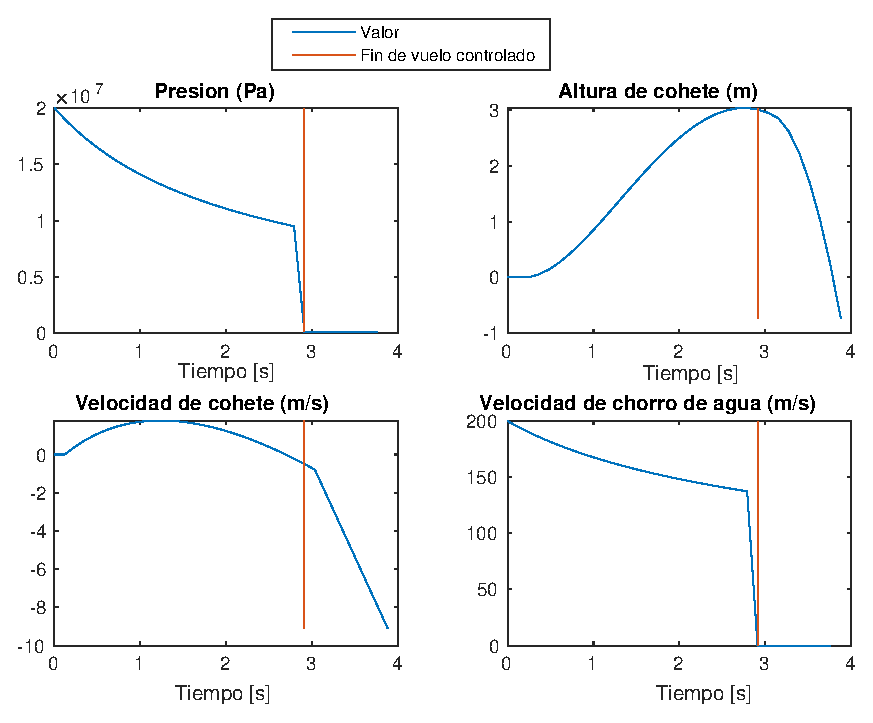
\includegraphics[width=0.8\linewidth]{fig/bottlerocket}
    \caption{Análisis preliminar para un vehículo propulsado por agua a presión. La presión es la del tanque (absoluta). El peso estructural que se utilizó fue de 10kg.}
    \label{fig:bottlerocket}
\end{figure}

Esto representa un vuelo de gran aceleración inicial, de mucha violencia, que dificulta la comprobación de sistemas en el que se tienen que modificar los parámetros de control y resolver los problemas de hardware que se vayan presentando. 

\subsection{Turbina a reacción}\label{ssec:turbina}
Se estudió la construcción de una turbina de combustible líquido como método de propulsión
del vehículo para poder comprobar el sistema de control, debido al excelente cociente de peso-empuje.

Esta idea se vio descartada por la complejidad asociada a la construcción de un elemento mecánico con constraints\todo{constrains} geométricos para alabes en múltiples dimensiones y balanceo a altas vueltas por minutos. Sumandosé a esto, no se tenía acceso al taller de la institución para poder realizar en tiempo y forma el dispositivo mecánico, que era la primer tarea inmediata a tener en banco de pruebas
asegurando su funcionamiento en optimas condiciones, para luego proseguir con el desarrollo
del vehículo y el sistema de control. Tampoco se contaba con las herramientas adecuadas para asegurar el éxito de la construcción dejando como opción acudir a prácticas no-convencionales con las herramientas existentes para generar el dispositivo.



\subsection{Propulsión eléctrica}\label{ssec:propelectrica}

\begin{figure}[htb]
    \centering
    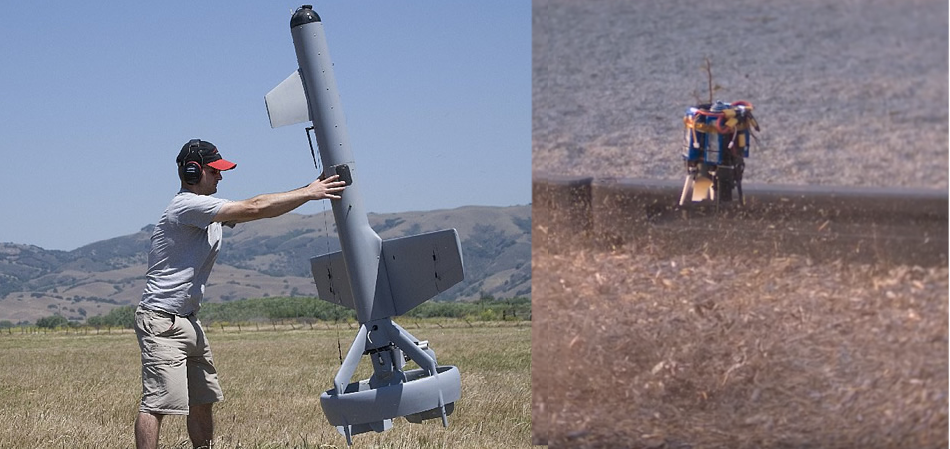
\includegraphics[width=0.8\linewidth]{fig/vbat_icarus.png}
    \caption{Dos vehículos VTVL eléctricos modernos. ``\href{https://www.navyrecognition.com/index.php/naval-news/naval-news-archive/2020/november/9260-company-martin-uav-demonstrates-shipboard-integration-with-its-v-bat-vtol-drone.html}{VBat}'' (Izq.) e ``\href{https://hackaday.com/2018/08/31/single-rotor-drone-a-thrust-vectoring-monocopter/}{Ikarus}'' (Der.).}
    \label{fig:vbat_icarus}
\end{figure}

Dadas las limitaciones de tiempo y alcance de un proyecto de la universidad se decidió por un diseño compuesto por elementos comercialmente disponibles.\footnote{\textit{Commercial off the shelf} (COTS)}

\medskip

Los vehículos VTVL eléctricos son propulsados por hélices en su mayoría y constan casi siempre de 4 o más propulsores en un arreglo simétrico y plano. Recientemente hay un interés por la construcción de vehículos de una sola hélice por la buena relación empuje--peso que tienen. Sin embargo, estos vehículos tienen sus complicaciones: 

\begin{itemize}
    \item La rotación dada al aire por la hélice causa un momento en el eje de propulsión que puede ser contrarrestado en vehículos multirrotores pero no asi en el caso de tener una sola hélice.
    \item Inclinar al rotor durante su funcionamiento causa una fuerza perpendicular a la dirección de inclinación conocido como el efecto giroscópico. 
\end{itemize}

El primer punto puede ser mitigado agregando álabes a la salida del flujo de aire por debajo del EDF (fan electrico con ducto) para modificar el flujo y contrarestar la rotación. El segundo punto se resuelve conociendo las ecuaciones de momento angular y controlando actuadores con un sistema de control a lazo cerrado. Los sistemas vistos en la figura~\ref{fig:vbat_icarus} suelen tener la particularidad de poder ser representados con relativa facilidad usando un solo marco de referencia sobre el vehículo para calcular las ecuaciones de momento angular.

\medskip

Existen placas pre-programadas para vehículos multirrotores, pero en el caso de vehículos monorrotores de hélice fija se precisa re-programar la placa para compensar el efecto giroscópico y agregar dinámica de álabes ya que no hay software disponible aún para esta configuración. En el caso de tener una hélice móvil se suma un nivel de complejidad agregada debido al despeje de las ecuaciones de momento angular (ver sección~\ref{sec:ecuacionesRigid}). Al momento de escribir este documento aún no hay desarrollo disponible de carácter público para esta configuración.

% \footnote{Agradecemos a \gls{lia} por hacerse cargo de la compra de los componentes faltantes que cayeron fuera del presupuesto necesarios para la fabricación del cohete.} 